%!TEX root = ../dissertation.tex
\chapter{Thermal conductance in high density graphene}
\label{ch:thermal_conductance_in_high_density_graphene}
In the high density, low temperature regime $(\mu >> k_BT)$, graphene has a well defined Fermi surface and the assumptions in Sommerfeld's derivation of the Lorentz ratio hold. 
Yigen lower bound on mobility is 35,000
Fong mobility about 5,000

\begin{figure}
\centering
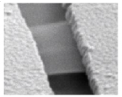
\includegraphics[height=45mm, valign=t]{figures/high_density_graphene/Yigen_picture.png}
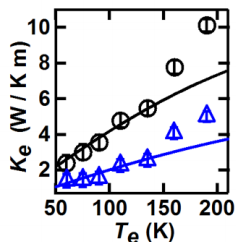
\includegraphics[height=50mm, valign=t]{figures/high_density_graphene/Yigen_Gth.png}
\caption{Electronic thermal conductivity of suspended graphene measured by Yigen et al. using resistive thermometry. Two curves correspond to different carrier densities. Solid lines are fits to the Wiedemann-Franz law. Below ${\sim150}~K$ the device shown WF behavior while at higher temperature the measured conduction is higher due to phonons coupling. Device is $650~nm$ long. Reprinted with permission from \cite{yigen_wiedemannfranz_2014}. Copyright (2014) American Chemical Society.}
\label{fig:Yigen}
\end{figure}


\begin{figure}
\centering
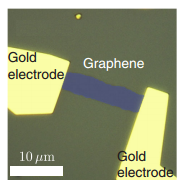
\includegraphics[height=45mm, valign=t]{figures/high_density_graphene/Fong_picture.png}
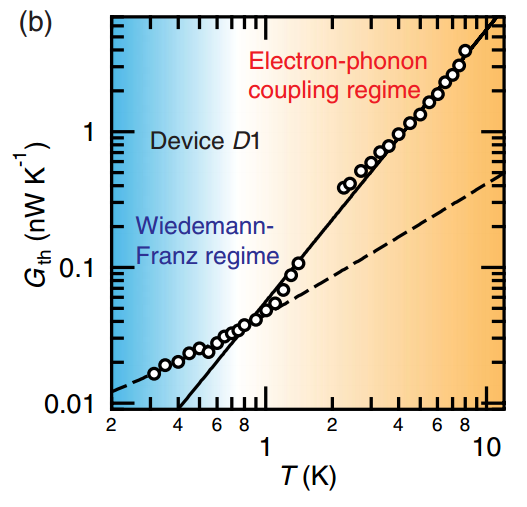
\includegraphics[height=50mm, valign=t]{figures/high_density_graphene/Fong_Gth.png}
\caption{Electronic thermal conductivity of graphene on $SiO_2$ measured by Fong et al. using Johnson noise thermometry. dashed line is a fit to the Wiedemann-Franz law. Below $1~K$ the device shown WF behavior while at higher temperature the measured conduction is higher due to phonons coupling. The longer device in this study results in phonons dominating conductance at a lower temperature. Reprinted under the Creative Commons Attribution 3.0 License from ref.~\cite{fong_measurement_2013}.}
\label{fig:Fong_Gth}
\end{figure}

\section{Device characteristics}
\begin{figure}
\centering
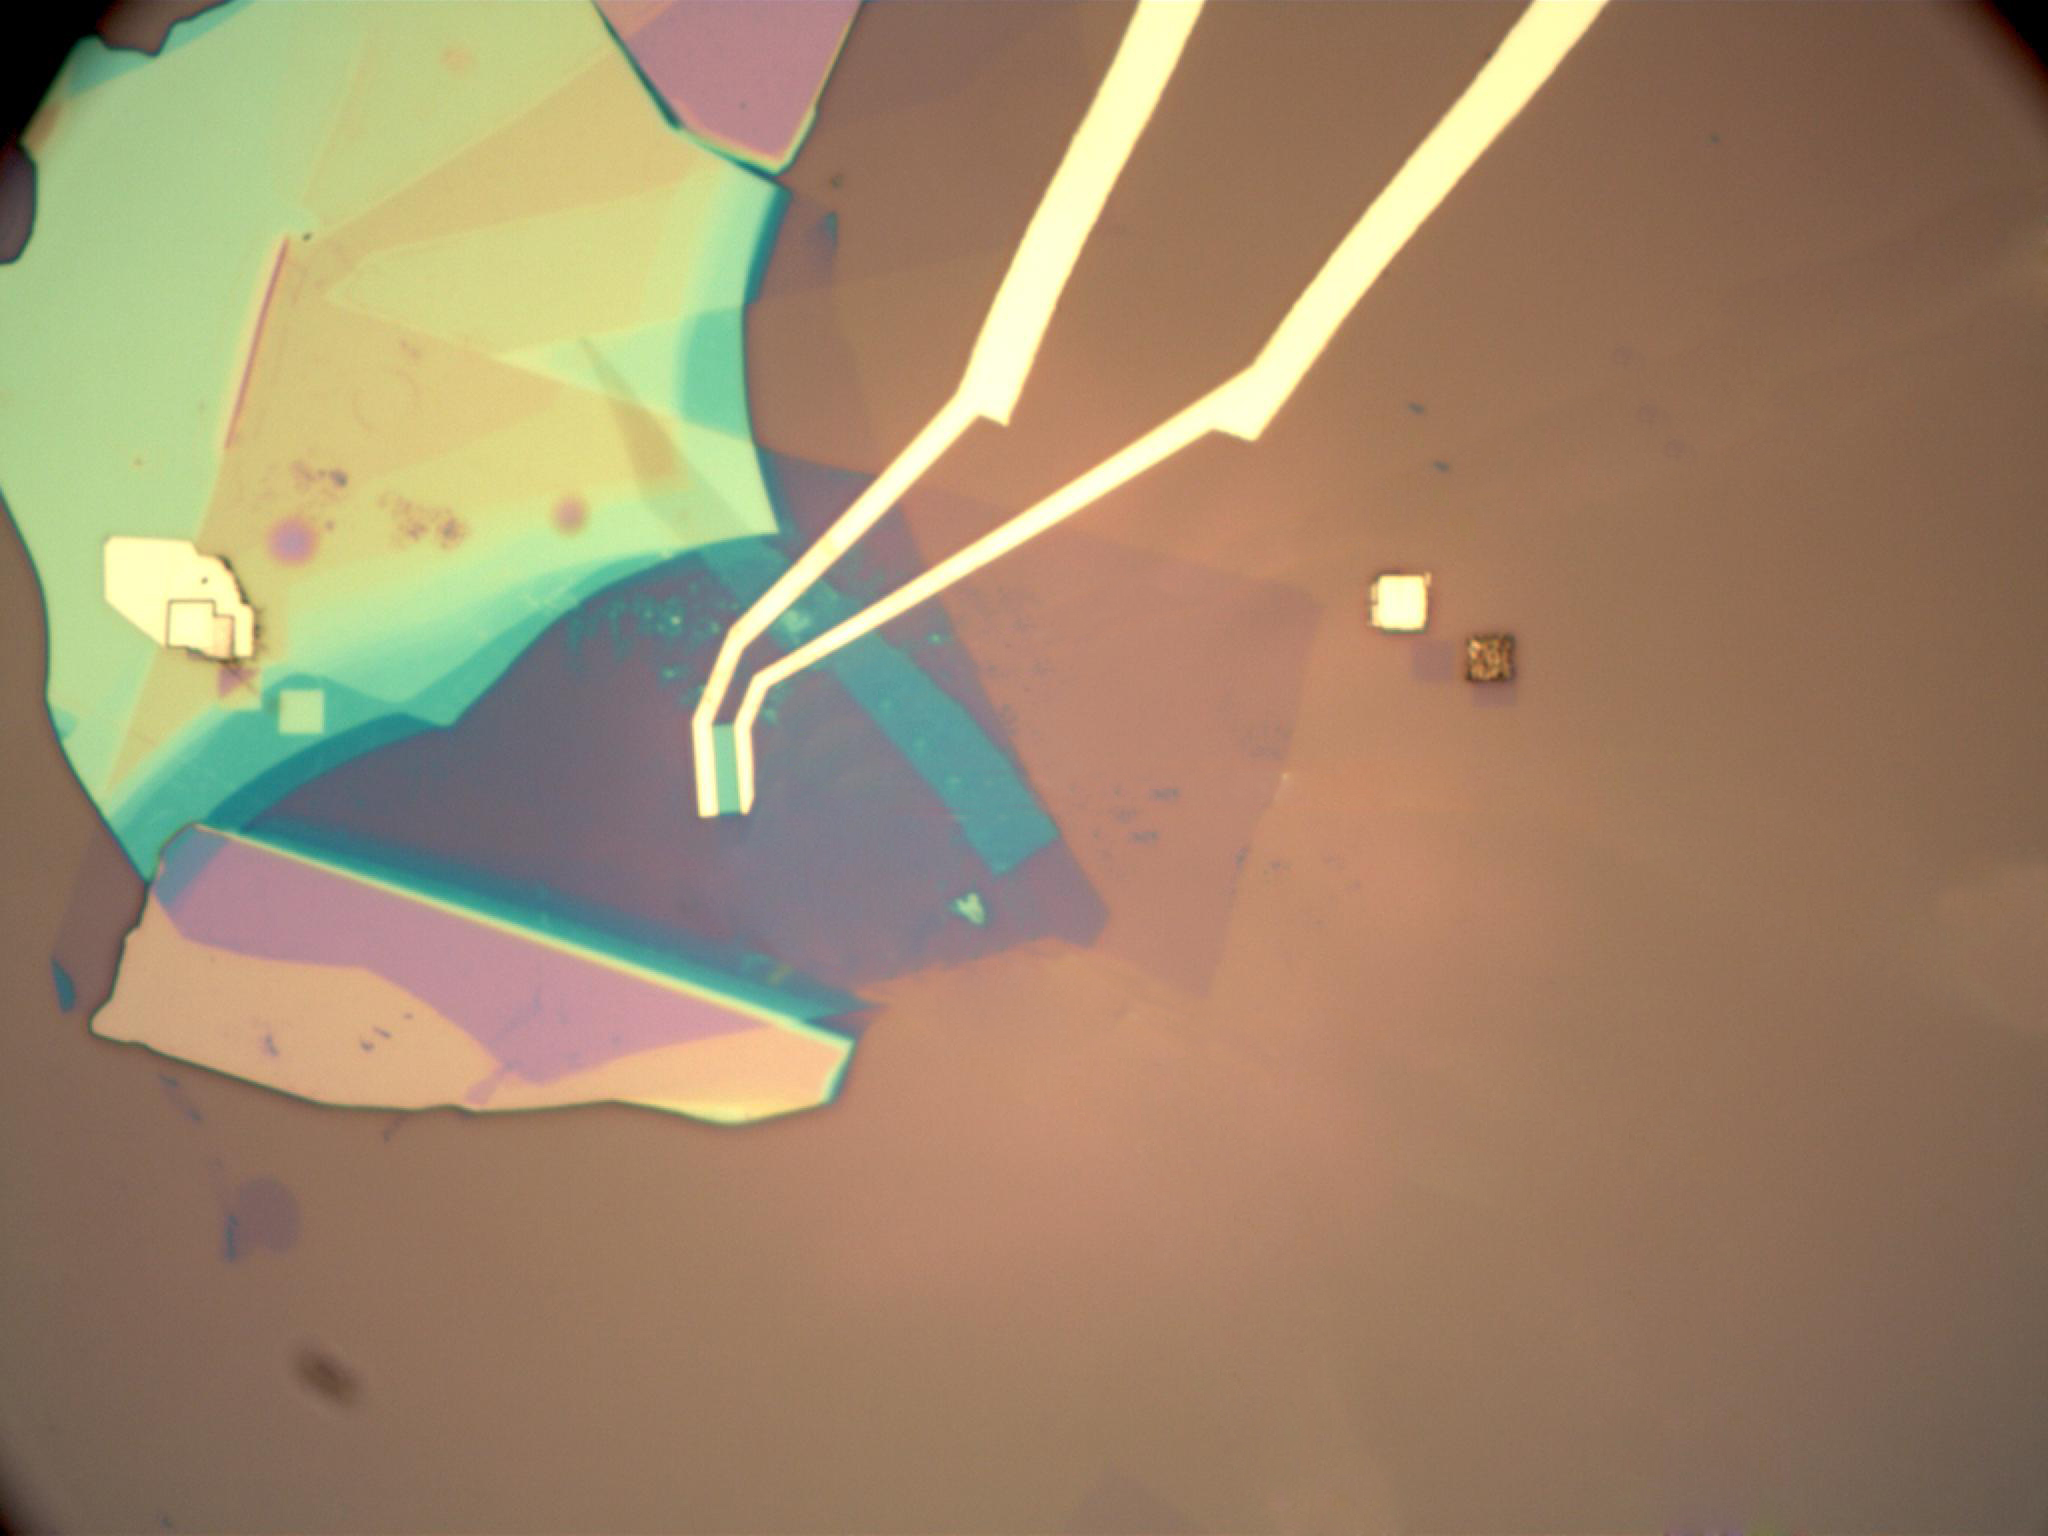
\includegraphics[height=45mm, valign=t]{figures/high_density_graphene/picture_aria.jpg}
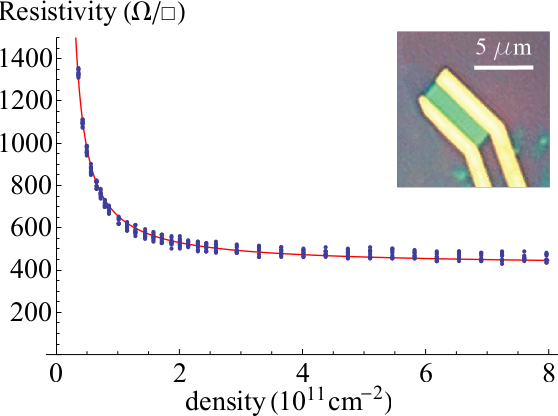
\includegraphics[height=50mm, valign=t]{figures/high_density_graphene/mobility.png}
\caption{(\textbf{left}) Microscope image of a two-terminal graphene device used in thermal conduction study $(2~\mu m\times6~\mu m)$. (\textbf{right}) Estimated resistivity vs carrier density from two-terminal resistance. Solid red line is a fit used to estimate a carrier mobility of $\mu\approx 350,000~cm^2/V~s$.
}
\label{fig:Aria}
\end{figure}


\section{Low temperature Wiedemann-Franz}

\section{High temperature electron-phonon}